% ----------------------------------------------------------------------- %
% Arquivo: cap2.tex
% ----------------------------------------------------------------------- %
\iffalse
==============<COMENTADO FORA>==============


\adESS{Conforme referenciado no Capítulo 1 o objetivo geral deste trabalho é implementar uma rede de sensores sem fio, baseada no conceito de SDN (Redes Definidas por Software) com fins de prover QoS para aplicações que se executam sobre a RSSF.}

\adESS{Um dos resultados esperados do mesmo é ganhar experiência com a aplicação de SDN em redes de Sensores e verificar as potencialidades de explorar este conceito em aplicações com requisitos de QoS. A plataforma SDN-WISE se apresenta como uma forma adequada para esta finalidade. Desta forma, inicialmente pretende-se implantar e analisar o comportamento de uma aplicação sobre a plataforma SDN-WISE no simulador Cooja e nos sensores Micaz. Embora já exista exemplos sobre o Cooja, a operacionalidade do mesmo sobre nodos reais deve ser avaliada.}


\adESS{Em um segundo momento, pretende-se conceber e implementar um controlador SDN que permita construir regras a partir de uma configuração estática de nodos e fluxos com requisitos de QoS associados a vazão e ao nível de bateria dos nodos.}


\adESS{A Figura \ref{modeloproposto} a seguir esboça uma primeira ideia desta estrutura:}

\begin{figure}[!htb]
    \centering
    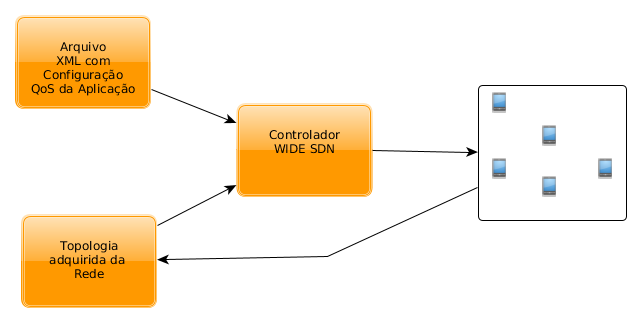
\includegraphics[width=13cm]{figs/DiagramaTCCAndre.png}
    \caption{Um Controlador direcionado a QoS}
    \label{modeloproposto}
\end{figure}

\adESS{Pretende-se conceber um controlador que, através de uma especificação em XML de uma aplicação, através de fluxos gerados em direção a um sorvedouro, e tendo como referência a topologia adquirida pelo SDN-WISE, forneça as regras de roteamento para a rede.}

\adESS{Neste ponto, também pretende-se avaliar a possibilidade de utilizar a visão \textit{statefull} proposta pelo SDN-WISE para ajustar o funcionamento do roteamento sem a necessidade de intervenção constante do Controlador.}

\adESS{Neste TCC não se terá inicialmente a preocupação de produzir um algoritmo ótimo para esta tarefa. O foco será em estabelecer a rede tendo como requisitos de banda e focando também o consumo de energia dos nodos. Como um dos problemas fundamentais em redes de sensores é a questão energética, pretende-se propor regras de roteamento que proporcionem a maximização da vida dos nodos ao mesmo tempo que garantam a banda na transmissão de fluxos que partem de nodos em direção aos sorvedouros.}

\adESS{Deve ser observado que o SDN-WISE permite capturar a topologia da rede, trazendo informações de vizinhos, SNRI e de nível de bateria de nodos. A questão de alocação de fluxos nos caminhos possíveis da rede exigirá um trabalho adicional de avaliação de banda disponível nos enlaces. Em adição, os nodos permitem ajustar a potência de transmissão. Tecnicamente é possível alterar as condições de conectividade da rede em função deste parâmetro. Uma fase de ajuste destas topologia usando esta possibilidade pode ser considerada.}

\adESS{Como continuidade desta etapa, pretende-se investigar a possibilidade de utilização da SDN no roteamento com múltiplos caminhos. Neste sentido, a ideia inicial é dispersar os fluxos através de caminhos disjuntos, expĺorando o roteamento multicaminho e reduzindo o esforço dos nodos em tempos de trabalho. Os requisitos de banda associados aos fluxos deverão ser cumpridos.}

\adESS{Novamente a preocupação aqui não é a confecção de algoritmos ótimos de roteamento, mas sim analisar a viabilidade do uso do sistema explorando regras que possibilitem o comportamento desejado e verificando possíveis problemas associados a esta abordagem.}

==============</COMENTADO FORA>==============
\fi

\chapter{Proposta}
\label{c_cap3}

%O presente trabalho propõe a implementação de uma rede de sensores sem fio, baseada no conceito de \ac{SDN}  para aplicações com requisitos \ac{QoS} que se executam sobre os nodos. Na sequência, a proposta é apresentada com mais detalhes e é apresentado um cronograma de execução.

As limitações de \textit{hardware} dos módulos das \ac{RSSF}s tornam o gerenciamento e a consequente garantia de \ac{QoS}, um desafio para os administradores da rede. Por isso, conforme referenciado no Capítulo \ref{c_introducao}, o objetivo geral deste trabalho é implementar uma rede de sensores sem fio, baseada no conceito de \ac{SDN} com fins de prover \ac{QoS} para aplicações que se executam sobre a \ac{RSSF}.

Para isso, o sistema \ac{SDN-WISE} será utilizado na comunicação entre as camadas da arquitetura \ac{SDN}. Na camada de dados, módulos MICAz que serão, em um primeiro momento, emulados no Cooja e, em seguida utilizados em um cenário real, ficam responsáveis por gerar e rotear os dados da rede. E na camada de controle, um algoritmo de roteamento será utilizado para oferecer garantias de vazão e baixo consumo energético para os módulos da camada de dados. Para tanto, o controlador terá acesso às informações dos módulos, da topologia da rede e dos requisitos de \ac{QoS} da aplicação, por conseguinte, o controlador aplicará as regras de roteamento, dinamicamente, na \ac{RSSF}.

\section{Detalhamento da proposta}

Para cumprir com os objetivos propostos, o trabalho será dividido em etapas de implantação de uma \ac{RSSF} baseada no conceito de \ac{SDN}. A primeira etapa tem como objetivo ganhar experiência com o protocolo \ac{SDN-WISE} e, implantar uma \ac{RSSF} com módulos MICAz. Para isso, a ferramenta de simulação de redes Cooja e módulos MICAz reais, serão utilizados para executar uma aplicação concebida para o trabalho. Já na segunda etapa, pretende-se verificar o potencial do conceito de \ac{SDN} em aplicações com requisitos de \ac{QoS}.

O Cooja permite simular os módulos MICAz, e utilizar o mesmo código (em linguagem C) desenvolvido para os módulos físicos no ambiente de simulação. Além do mais, o Cooja disponibiliza várias ferramentas que auxiliam na depuração do código e na criação de cenários com grande quantidades de módulos. A Figura \ref{simuladorCooja}, mostra algumas das principais ferramentas. A \textit{Network} permite a visualização da troca de pacotes e, o posicionamento dos módulos, de forma gráfica. Já as ferramentas \textit{Mote Output} e \textit{Radio messages}, registram, respectivamente, os \textit{logs} publicados pelos módulos e as mensagens transmitidas através dos seus rádios. Na \textit{Timeline}, é possível observar as transmissões realizadas. Por fim, o Cooja oferece uma interface \ac{TCP} que, pode ser acessada, através de um terminal externo. O que, neste trabalho, permite a integração do controlador com os módulos simulados. Por estas razões, escolheu-se trabalhar com esta ferramenta para implantar uma \ac{RSSF}, baseado no conceito de \ac{SDN}.

\begin{figure}[!htb]
    \centering
    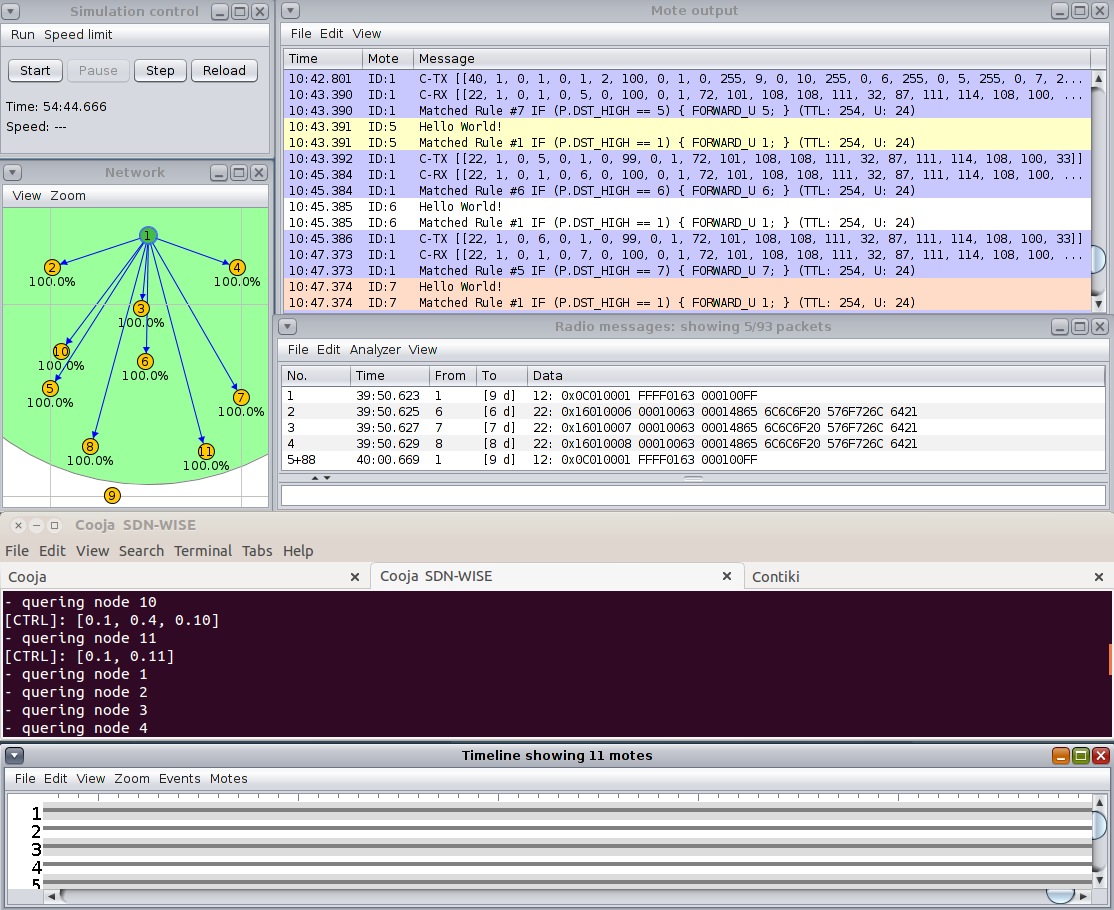
\includegraphics[width=15cm]{figs/simuladorCooja.png}
    \caption{Visão geral do simulador de redes Cooja.}
    \label{simuladorCooja}
\end{figure}

Dessa forma, na primeira etapa, será utilizado um experimento básico, disponibilizado pelos autores do \ac{SDN-WISE} para o Cooja. Neste exemplo, um controlador, desenvolvido em Java, utiliza o algoritmo de Dijkstra para encontrar os caminhos com menor custo. Os módulos (\textit{sink} e \textit{source}), também desenvolvidos em Java, utilizam os caminhos recebidos pelo controlador para rotear os pacotes, gerados de forma aleatória, até o único \textit{sink} da rede. Em seguida, ainda na primeira etapa, pretende-se implantar e analisar o comportamento de uma aplicação sobre a plataforma \ac{SDN-WISE} no Cooja, utilizando sensores MICAz emulados. Embora já exista o exemplo disponibilizado, a operacionalidade do mesmo sobre módulos MICAz deve ser avaliada, uma vez que os módulos (\textit{sink} e \textit{source}) disponibilizados, são genéricos, ou seja, não foram projetados de acordo com as características de \textit{hardware} do MICAz. 

O foco da segunda etapa de desenvolvimento é explorar o conceito de \ac{SDN} em aplicações com requisitos de \ac{QoS}. Para isso, o controlador utilizado na primeira etapa deverá ser modificado. A ideia é que ele possibilite a configuração estática dos módulos e, dos fluxos que possuem requisitos de \ac{QoS} associados à vazão e, ao nível de bateria dos nodos. Além disso, o algoritmo de Dijkstra, padrão do controlador, será substituído por um que faça a alocação de fluxos a caminhos da rede de forma a atender aos requisitos de vazão e consumo energético da aplicação. 

Além das modificações no controlador, outra medidas podem ser implementadas com objetivo de garantir eficiência energética e a largura de banda exigida pela aplicação da rede \ac{SDN}. Por exemplo, pretende-se verificar a possibilidade do uso dos estados, propostos pelo \ac{SDN-WISE}, para alterar o roteamento, sem a necessidade de intervenção constante do controlador e, garantir o tráfego de dados na rede, como mostrado na Seção \ref{s_c2_wise_sdn_QOS}. Pode-se, ainda, utilizar a capacidade, do \ac{SDN-WISE}, de ajuste da potência de transmissão dos módulos, para modificar a topologia da rede, uma vez que, a alteração deste parâmetro impacta diretamente nas condições de conectividade da rede.

Para esta etapa, planeja-se também, verificar a melhor forma de avaliação da largura de banda disponível para cada enlace e, como alocar caminhos com banda disponível para fluxos com exigências de \ac{QoS}. Por fim, pretende-se investigar a possibilidade do uso de algoritmos de roteamento por múltiplos caminhos em \ac{RSSF}s baseadas no conceito de \ac{SDN}. Neste sentido, a ideia inicial é dispersar os fluxos através de caminhos disjuntos, explorando o roteamento multicaminho e reduzindo o esforço dos nodos em tempos de trabalho. 

Assim, pretende-se, ao fim deste trabalho, apresentar a estrutura mostrada na Figura \ref{Arch_wiseSDN_TCC}. A partir dela observa-se que o controlador utiliza as configurações recebidas, através de um arquivo \ac{XML}, em conjunto com informações dos módulos e da topologia da rede para criar regras de roteamento. É importante mencionar que, o foco deste trabalho não é propor um algoritmo ótimo para garantia de \ac{QoS} em aplicações da \ac{RSSF}. Mas sim, analisar a viabilidade do uso do conceito de \ac{SDN}, para atender aos requisitos de \ac{QoS} das aplicações das \ac{RSSF}s e, explorar regras de roteamento, que garantam a maximização da vida dos nodos, ao mesmo tempo que garantam a banda na transmissão de fluxos que, partem de nodos em direção aos sorvedouros da rede.


\begin{figure}[!htb]
    \centering
    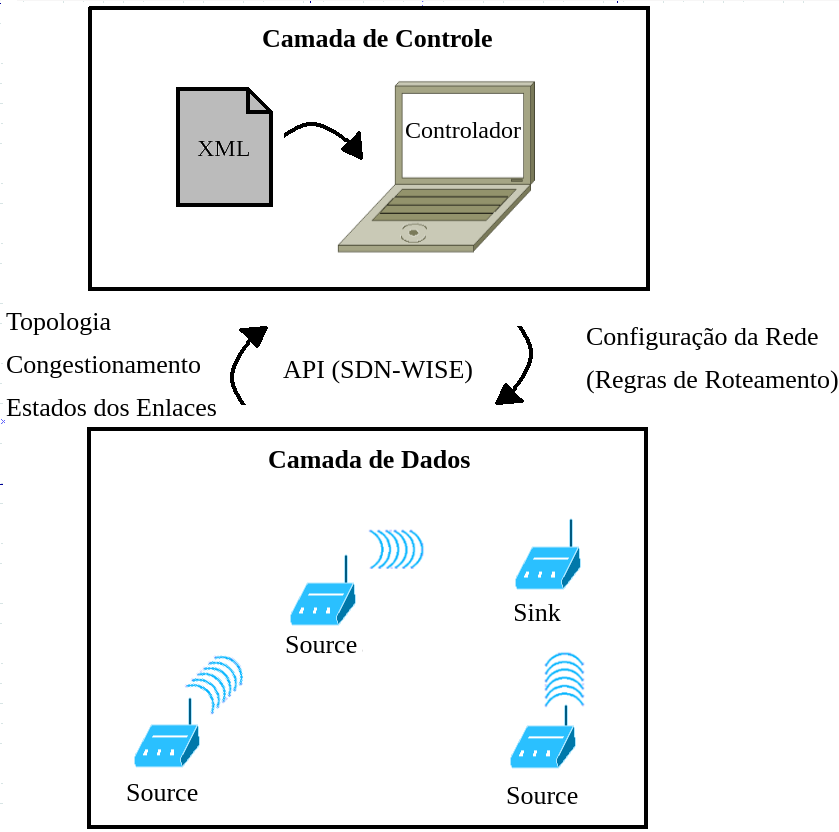
\includegraphics[width=6cm]{figs/Arch_wiseSDN_TCC.png}
    \caption{Arquitetura \ac{SDN} na \ac{RSSF} para garantia de \ac{QoS}}
    \label{Arch_wiseSDN_TCC}
\end{figure}

\section{Recursos, Etapas e Cronograma}

\subsection{Recursos necessários}

\begin{figure*}[t!]
    \centering
    \begin{subfigure}[t]{0.45\textwidth}
        \centering
        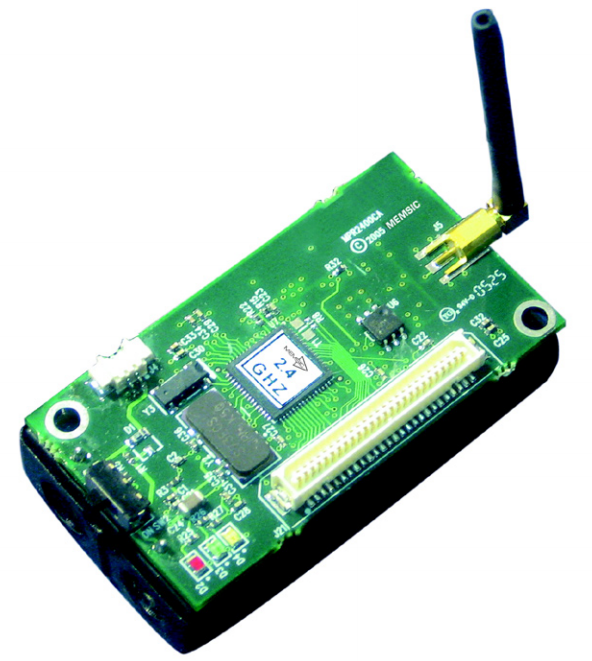
\includegraphics[width=4cm]{figs/ModulosMICAZ.png}
        \caption{Mote MICAz. \cite{micaz2013wireless}}
        \label{ModulosMICAZ}
    \end{subfigure}%
    ~ 
    \begin{subfigure}[t]{0.45\textwidth}
        \centering
        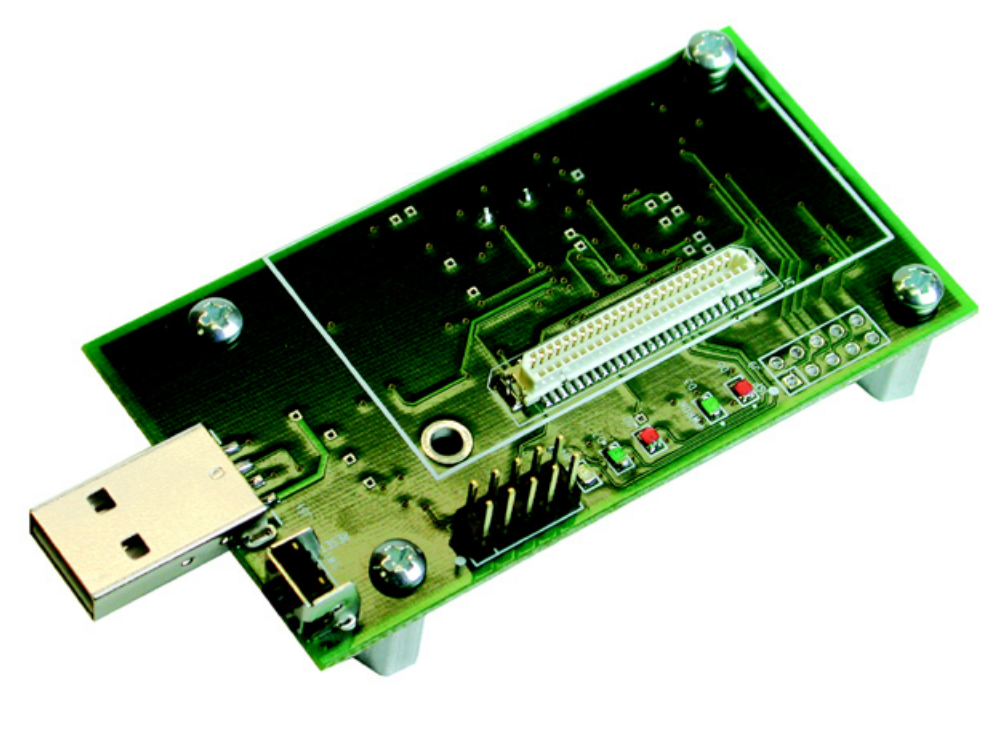
\includegraphics[width=4cm]{figs/InterfaceMICAZ.png}
        \caption{Interface de programação para MICAz. \cite{micaz2013wireless}}
        \label{InterfaceMICAZ}
    \end{subfigure}
    \caption{MICAz e programadora necessária para o trabalho.}
\end{figure*}

O controlador da arquitetura \ac{SDN}, será executado em um \textit{laptop}, e os módulos \textit{sink} e \textit{source} serão implementados com módulos MICAz (Figura \ref{ModulosMICAZ}). Porém, o \textit{sink} será conectado ao \textit{laptop} através da sua interface de programação (Figura \ref{InterfaceMICAZ})


\subsection{Etapas de desenvolvimento}
\begin{itemize}  
    \item Implantação, no Cooja, de uma \ac{RSSF} com arquitetura \ac{SDN}, utilizando o controlador e, módulos \textit{sink} e \textit{source} disponibilizados pelos autores do \ac{SDN-WISE}.
    \item Migração do código dos módulos genéricos para a plataforma MICAz.
    \item Estudo e implementação de uma aplicação piloto.
    \item Análise e implementação de algoritmos de roteamento para \ac{RSSF}s que, ofereçam garantia de vazão e/ou eficiência energética, para a aplicação piloto.
    \item Criar um cenário real com módulo MICAz físicos.
    \item Avaliação do comportamento da \ac{RSSF} implantada no cenário real. 
\end{itemize}

\subsection{Cronograma}

O cronograma mostrado na Tabela \ref{t_cronograma} será seguido, com o objetivo de implantar uma \ac{RSSF}, baseada no \ac{SDN-WISE} para provimento de \ac{QoS}. Cada etapa de desenvolvimento descrita anteriormente será realizada, em pelo menos, duas semanas. Porém, será realizado o acompanhamento semanal, de acordo com abordagens de gestão, como o Kanban. Como visto na tabela, exceto pela escrita e correção do texto, todas as etapas devem ser feitas separadamente, e na sequência que garanta a implementação da etapa seguinte.


\begin{table}[!htpb]
\centering
\begin{small}
  \setlength{\tabcolsep}{3pt}
\begin{tabular}{|c|c|c|c|c|c|c|c|c|c|c|c|c|}\hline
 & \multicolumn{12}{c|}{Mês/Semanas}\\ \cline{2-13}
\raisebox{1.5ex}{Etapa} & Jul & Jul & Ago & Ago & Set & Set & Out & Out & Nov & Nov & Dez & Dez \\ 
                        & 1-2 & 3-4 & 1-2 & 3-4 & 1-2 & 3-4 & 1-2 & 3-4 & 1-2 & 3-4 & 1-2 & 3-4 \\\hline

% exemplo de linha
% 1 & & & & & & & & & & & & \\ \hline

Implantação no Cooja      & X & & & & & & & & & & & \\ \hline
Migração para o MICAz     & & X & X & & & & & & & & & \\ \hline
Aplicação Piloto          & & & & X & & & & & & & & \\ \hline
Algoritmos                & & & & & X & X & & & & & & \\ \hline
Escrita do TCC2           & & & X & X & X & X &  & & & & &  \\ \hline
Cenário Real              & & & & & & & X & X & X & & &  \\ \hline
Avaliação                 & & & & & & & & & & X & &  \\ \hline
Correções do Texto        & & & & & & & X & X & X & X & &  \\ \hline
Entrega da Monografia     & & & & & & & & & & & X &  \\ \hline
Apresentação à banca      & & & & & & & & & & & X &  \\ \hline
Correções e Entrega Final & & & & & & & & & & & & X \\ \hline

\end{tabular} 
\end{small}
\caption{Cronograma das atividades previstas}
\label{t_cronograma}
\end{table} 
